% 
% File:	  test14.qasm
% Date:	  22-Mar-04
% Author: I. Chuang <ichuang@mit.edu>
%
% Sample qasm input file - three-qubit FT QEC
% circuit with syndrome measurement
% 
% 	defbox	synd,4,0,'\txt{Process\\Syndrome}'
% 	defbox	rop,7,4,'{\cal R}'
% 
% 	qubit	q0	% code data qubits
% 	qubit	q1
% 	qubit	q2
% 	qubit	s0,0	% syndrome measurement qubits
% 	qubit	s1,0
% 	cbit	c0,0	% classical bits to store syndromes
% 	cbit	c1,0
% 
% 	h	s0	% create EPR pair for FT meas
% 	cnot	s0,s1
% 	cnot	q0,s0	% measure parity of q0,q1
% 	nop	s1	% prevent cnot's from colliding
% 	cnot	q1,s1
% 	cnot	s0,s1	% uncreate EPR
% 	h	s0
% 	measure	s0	% measure syndrome qubits
% 	nop	s1
% 	measure s1
% 	cnot	s0,c0	% copy to classical bits
% 	nop	s1
% 	cnot	s1,c1
% 	space	s0
% 
% 	zero	s0
% 	zero	s1
% 	h	s0	% create EPR pair for FT meas
% 	cnot	s0,s1
% 	cnot	q1,s0	% measure parity of q1,q2
% 	nop	s1	% prevent cnot's from colliding
% 	cnot	q2,s1
% 	cnot	s0,s1	% uncreate EPR
% 	h	s0
% 	measure	s0	% measure syndrome qubits
% 	nop	s1
% 	measure s1
% 
% 	synd	s0,s1,c0,c1
% 	rop	s0,s1,c0,c1,q0,q1,q2

%  Time 01:
%    Gate 00 h(s0)
%  Time 02:
%    Gate 01 cnot(s0,s1)
%  Time 03:
%    Gate 02 cnot(q0,s0)
%    Gate 03 nop(s1)
%  Time 04:
%    Gate 04 cnot(q1,s1)
%  Time 05:
%    Gate 05 cnot(s0,s1)
%  Time 06:
%    Gate 06 h(s0)
%    Gate 08 nop(s1)
%  Time 07:
%    Gate 07 measure(s0)
%    Gate 09 measure(s1)
%  Time 08:
%    Gate 10 cnot(s0,c0)
%    Gate 11 nop(s1)
%  Time 09:
%    Gate 12 cnot(s1,c1)
%    Gate 13 space(s0)
%  Time 10:
%    Gate 14 zero(s0)
%    Gate 15 zero(s1)
%  Time 11:
%    Gate 16 h(s0)
%  Time 12:
%    Gate 17 cnot(s0,s1)
%  Time 13:
%    Gate 18 cnot(q1,s0)
%    Gate 19 nop(s1)
%  Time 14:
%    Gate 20 cnot(q2,s1)
%  Time 15:
%    Gate 21 cnot(s0,s1)
%  Time 16:
%    Gate 22 h(s0)
%    Gate 24 nop(s1)
%  Time 17:
%    Gate 23 measure(s0)
%    Gate 25 measure(s1)
%  Time 18:
%    Gate 26 synd(s0,s1,c0,c1)
%  Time 19:
%    Gate 27 rop(s0,s1,c0,c1,q0,q1,q2)

% Qubit circuit matrix:
%
% q0: n  , n  , gCA, n  , n  , n  , n  , n  , n  , n  , n  , n  , n  , n  , n  , n  , n  , n  , gSA, n  
% q1: n  , n  , n  , gDB, n  , n  , n  , n  , n  , n  , n  , n  , gMB, n  , n  , n  , n  , n  , gSB, n  
% q2: n  , n  , n  , n  , n  , n  , n  , n  , n  , n  , n  , n  , n  , gNC, n  , n  , n  , n  , gSC, n  
% s0: gAD, gBD, gCD, n  , gED, gFD, gGD, gHD, gID, gJD, gKD, gLD, gMD, n  , gOD, gPD, gQD, gRD, gSD, N  
% s1: n  , gBE, gCE, gDE, gEE, gFE, gGE, gHE, gIE, gJE, n  , gLE, gME, gNE, gOE, gPE, gQE, gRE, gSE, N  
% c0: N  , N  , N  , N  , N  , N  , N  , gHF, N  , N  , N  , N  , N  , N  , N  , N  , N  , gRF, gSF, N  
% c1: N  , N  , N  , N  , N  , N  , N  , N  , gIG, N  , N  , N  , N  , N  , N  , N  , N  , gRG, gSG, N  

\documentclass[11pt]{article}
%
% File:   xyqcirc.tex
% Date:   14-Mar-04
% Author: I. Chuang <ichuang@mit.edu>
%
% Definitions for producing quantum circuits with XYPIC in latex
%
% $Log: xyqcirc.tex,v $
% Revision 1.17  2004/03/25 05:01:23  ike
% discard and slash
%
% Revision 1.16  2004/03/25 04:58:42  ike
% added discard, and variable width dmeter
%
% Revision 1.15  2004/03/24 23:43:33  ike
% \dmeter and \sq
%
% Revision 1.14  2004/03/24 20:29:40  ike
% added \t for swap
%
% Revision 1.13  2004/03/24 17:52:16  ike
% removed \w from \gspace
%
% Revision 1.12  2004/03/24 16:38:34  ike
% added small space before |0> for \z
%
% Revision 1.11  2004/03/24 16:23:11  ike
% added \z
%
% Revision 1.10  2004/03/24 16:19:11  ike
% added multiple qubit operations
%
% Revision 1.9  2004/03/24 03:03:44  ike
% typo
%
% Revision 1.8  2004/03/24 02:50:09  ike
% added qv
%
% Revision 1.7  2004/03/24 00:07:34  ike
% add \m matrix op
%
% Revision 1.6  2004/03/23 23:13:10  ike
% misc
%
% Revision 1.5  2004/03/23 23:12:42  ike
% works now
%
% Revision 1.4  2004/03/23 22:22:34  ike
% ifthen also failes - because xymatrix entries in \save...\restore
%
% Revision 1.3  2004/03/23 21:34:36  ike
% no q/c wire switching
%
% Revision 1.2  2004/03/23 21:25:29  ike
% classical qo quantum wire switching try
%
% Revision 1.1  2004/03/23 21:01:46  ike
% Initial revision
%

%%%%%%%%%%%%%%%%%%%%%%%%%%%%%%%%%%%%%%%%%%%%%%%%%%%%%%%%%%%%%%%%%%%%%%%%%%%%%
% preliminaries

\usepackage{graphicx}
%\usepackage{epstopdf}
\usepackage[frame,line,arrow,matrix,tips]{xy}	% all that is usually necessary
\CompilePrefix{xygui-}
\makeindex
\pagestyle{empty}

\setlength{\oddsidemargin}{-0.5in}	% 1.25in left margin 
\setlength{\evensidemargin}{-0.5in}	% 1.25in left margin (even pages)

\setlength{\topmargin}{0.0in}		% 1in top margin
\setlength{\textwidth}{6.25in}		% 6.0in text - 1.25in rt margin
\setlength{\textheight}{8.6in}		% Body ht for 1in margins
\addtolength{\topmargin}{-\headheight}	% No header, so compensate
\addtolength{\topmargin}{-\headsep}	% for header height and separation

\begin{document}

\thispagestyle{empty}

%%%%%%%%%%%%%%%%%%%%%%%%%%%%%%%%%%%%%%%%%%%%%%%%%%%%%%%%%%%%%%%%%%%%%%%%%%%%%
% wires

\def\w{\ar@{-}[l]}
\def\W{\ar@{=}[l]}

%%%%%%%%%%%%%%%%%%%%%%%%%%%%%%%%%%%%%%%%%%%%%%%%%%%%%%%%%%%%%%%%%%%%%%%%%%%%%
% labels

% simple label
\def\A#1{\save []="#1" \restore}

%%%%%%%%%%%%%%%%%%%%%%%%%%%%%%%%%%%%%%%%%%%%%%%%%%%%%%%%%%%%%%%%%%%%%%%%%%%%%
% single qubit operations

\def\op#1{*+[F]{\rule[-0.2ex]{0ex}{2.1ex}#1}}	% operator in box
\def\b{*={\bullet}}
\def\o{*={\oplus}}
\def\t{*={\times}}				% for swap gate
\def\sq{*=<6pt,6pt>[F]{}}			% square, for controlled-phase
\def\m#1{\left[\matrix{#1}\right]}		% matrix shortcut
\def\z{*+[]{\rule[-0.2ex]{0ex}{2.1ex}~|0\>}}	% re-init to |0>
\def\discard{*[]{\rule[-0.2ex]{0.75pt}{2.1ex}~}}	% vertical ``|''
\def\slash{*={/}}				% slash for wire bundles

%%%%%%%%%%%%%%%%%%%%%%%%%%%%%%%%%%%%%%%%%%%%%%%%%%%%%%%%%%%%%%%%%%%%%%%%%%%%%
% nop's

\def\N{*-{}\W}
\def\n{*-{}\w}

%%%%%%%%%%%%%%%%%%%%%%%%%%%%%%%%%%%%%%%%%%%%%%%%%%%%%%%%%%%%%%%%%%%%%%%%%%%%%
% misc definitions

\def\>{\rangle}
\def\<{\langle}
\def\ua{\uparrow}

% measurement box
\def\meter{*+[]{\put(-3,0){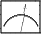
\includegraphics[scale=.5]{meter.png}}~~~~}%
		\ar@{-}[l]}

%%%%%%%%%%%%%%%%%%%%%%%%%%%%%%%%%%%%%%%%%%%%%%%%%%%%%%%%%%%%%%%%%%%%%%%%%%%%%
% qubit names (and also revert to qubit wires, vs, cbit wires)

\def\q#1{*+{\rule[-0.2ex]{0ex}{2.1ex}|#1\>}}
\def\qv#1#2{*+{\rule[-0.2ex]{0ex}{2.1ex}|#1\>=|#2\>}}
	
%%%%%%%%%%%%%%%%%%%%%%%%%%%%%%%%%%%%%%%%%%%%%%%%%%%%%%%%%%%%%%%%%%%%%%%%%%%%%
% multiple qubit gates

% utulity text box for figuring out width of things
\newbox{\sbox}

% empty space of width determined by the text argument
\def\gspace#1{*+{\rule[-0.2ex]{0ex}{2.1ex}%
	\setbox\sbox=\hbox{$#1$}%
	\hspace*{\wd\sbox}}}
	
% n-qubit operation #1=box label, #2=number of qubits (eg d=2 qubits, ddd=4)
\def\gnqubit#1#2{\gspace{#1}
		 \save [].[#2]!C="qq"*[F]\frm{}\restore
		 \save "qq"*[]{#1} \restore}

% two-qubit operation
\def\gtwo#1{\gnqubit{#1}{d}}

% two-qubit operation
\def\gthree#1{\gnqubit{#1}{dd}}

%%%%%%%%%%%%%%%%%%%%%%%%%%%%%%%%%%%%%%%%%%%%%%%%%%%%%%%%%%%%%%%%%%%%%%%%%%%%%
% ``D'' style measurement gate a-la-cleve, at Michael Nielsen's request

\def\dmeterwide#1#2{*{\xy <0pt,-8pt>;<0pt,8pt> **@{-};
		    <0pt,-8pt>;<#2,-8pt> **@{-} ;
		    <0pt, 8pt>;<#2, 8pt> **@{-} ;
		    <#2,0pt>-<5pt,0pt>*{#1} ;
		    <#2,0pt>*\cir<8pt>{r_l}\endxy}}

\def\dmeter#1{\dmeterwide{#1}{12pt}}

%%%%%%%%%%%%%%%%%%%%%%%%%%%%%%%%%%%%%%%%%%%%%%%%%%%%%%%%%%%%%%%%%%%%%%%%%%%%%


% definitions for the circuit elements

\def\gAD{\op{H}\w\A{gAD}}
\def\gBD{\b\w\A{gBD}}
\def\gBE{\o\w\A{gBE}}
\def\gCA{\b\w\A{gCA}}
\def\gCD{\o\w\A{gCD}}
\def\gCE{*-{}\w\A{gCE}}
\def\gDB{\b\w\A{gDB}}
\def\gDE{\o\w\A{gDE}}
\def\gED{\b\w\A{gED}}
\def\gEE{\o\w\A{gEE}}
\def\gFD{\op{H}\w\A{gFD}}
\def\gGD{\meter\w\A{gGD}}
\def\gFE{*-{}\w\A{gFE}}
\def\gGE{\meter\w\A{gGE}}
\def\gHD{\b\W\A{gHD}}
\def\gHF{\o\W\A{gHF}}
\def\gHE{*-{}\W\A{gHE}}
\def\gIE{\b\W\A{gIE}}
\def\gIG{\o\W\A{gIG}}
\def\gID{\A{gID}}
\def\gJD{\z\A{gJD}}
\def\gJE{\z\A{gJE}}
\def\gKD{\op{H}\w\A{gKD}}
\def\gLD{\b\w\A{gLD}}
\def\gLE{\o\w\A{gLE}}
\def\gMB{\b\w\A{gMB}}
\def\gMD{\o\w\A{gMD}}
\def\gME{*-{}\w\A{gME}}
\def\gNC{\b\w\A{gNC}}
\def\gNE{\o\w\A{gNE}}
\def\gOD{\b\w\A{gOD}}
\def\gOE{\o\w\A{gOE}}
\def\gPD{\op{H}\w\A{gPD}}
\def\gQD{\meter\w\A{gQD}}
\def\gPE{*-{}\w\A{gPE}}
\def\gQE{\meter\w\A{gQE}}
\def\gRD{\gnqubit{\txt{Process\\Syndrome}}{ddd}\W\A{gRD}}
\def\gRE{\gspace{\txt{Process\\Syndrome}}\W\A{gRE}}
\def\gRF{\gspace{\txt{Process\\Syndrome}}\W\A{gRF}}
\def\gRG{\gspace{\txt{Process\\Syndrome}}\W\A{gRG}}
\def\gSA{\gnqubit{{\cal R}}{dd}\w\A{gSA}}
\def\gSB{\gspace{{\cal R}}\w\A{gSB}}
\def\gSC{\gspace{{\cal R}}\w\A{gSC}}
\def\gSD{\b\W\A{gSD}}
\def\gSE{\b\W\A{gSE}}
\def\gSF{\b\W\A{gSF}}
\def\gSG{\b\W\A{gSG}}

% definitions for bit labels and initial states

\def\bA{ \q{q_{0}}}
\def\bB{ \q{q_{1}}}
\def\bC{ \q{q_{2}}}
\def\bD{\qv{s_{0}}{0}}
\def\bE{\qv{s_{1}}{0}}
\def\bF{   {c_{0} = 0}}
\def\bG{   {c_{1} = 0}}

% The quantum circuit as an xymatrix

\xymatrix@R=5pt@C=10pt{
    \bA & \n   &\n   &\gCA &\n   &\n   &\n   &\n   &\n   &\n   &\n   &\n   &\n   &\n   &\n   &\n   &\n   &\n   &\n   &\gSA &\n  
\\  \bB & \n   &\n   &\n   &\gDB &\n   &\n   &\n   &\n   &\n   &\n   &\n   &\n   &\gMB &\n   &\n   &\n   &\n   &\n   &\gSB &\n  
\\  \bC & \n   &\n   &\n   &\n   &\n   &\n   &\n   &\n   &\n   &\n   &\n   &\n   &\n   &\gNC &\n   &\n   &\n   &\n   &\gSC &\n  
\\  \bD & \gAD &\gBD &\gCD &\n   &\gED &\gFD &\gGD &\gHD &\gID &\gJD &\gKD &\gLD &\gMD &\n   &\gOD &\gPD &\gQD &\gRD &\gSD &\N  
\\  \bE & \n   &\gBE &\gCE &\gDE &\gEE &\gFE &\gGE &\gHE &\gIE &\gJE &\n   &\gLE &\gME &\gNE &\gOE &\gPE &\gQE &\gRE &\gSE &\N  
\\  \bF & \N   &\N   &\N   &\N   &\N   &\N   &\N   &\gHF &\N   &\N   &\N   &\N   &\N   &\N   &\N   &\N   &\N   &\gRF &\gSF &\N  
\\  \bG & \N   &\N   &\N   &\N   &\N   &\N   &\N   &\N   &\gIG &\N   &\N   &\N   &\N   &\N   &\N   &\N   &\N   &\gRG &\gSG &\N  
%
% Vertical lines and other post-xymatrix latex
%
\ar@{-}"gBE";"gBD"
\ar@{-}"gCD";"gCA"
\ar@{-}"gDE";"gDB"
\ar@{-}"gEE";"gED"
\ar@{=}"gHF";"gHD"
\ar@{=}"gIG";"gIE"
\ar@{-}"gLE";"gLD"
\ar@{-}"gMD";"gMB"
\ar@{-}"gNE";"gNC"
\ar@{-}"gOE";"gOD"
\ar@{=}"gSC";"gSD"\ar@{=}"gSC";"gSE"\ar@{=}"gSC";"gSF"\ar@{=}"gSC";"gSG"
}

\end{document}
